\documentclass[journal, a4paper]{IEEEtran}

% some very useful LaTeX packages include:

%\usepackage{cite}      % Written by Donald Arseneau
                        % V1.6 and later of IEEEtran pre-defines the format
                        % of the cite.sty package \cite{} output to follow
                        % that of IEEE. Loading the cite package will
                        % result in citation numbers being automatically
                        % sorted and properly "ranged". i.e.,
                        % [1], [9], [2], [7], [5], [6]
                        % (without using cite.sty)
                        % will become:
                        % [1], [2], [5]--[7], [9] (using cite.sty)
                        % cite.sty's \cite will automatically add leading
                        % space, if needed. Use cite.sty's noadjust option
                        % (cite.sty V3.8 and later) if you want to turn this
                        % off. cite.sty is already installed on most LaTeX
                        % systems. The latest version can be obtained at:
                        % http://www.ctan.org/tex-archive/macros/latex/contrib/supported/cite/

\usepackage{graphicx}   % Written by David Carlisle and Sebastian Rahtz
                        % Required if you want graphics, photos, etc.
                        % graphicx.sty is already installed on most LaTeX
                        % systems. The latest version and documentation can
                        % be obtained at:
                        % http://www.ctan.org/tex-archive/macros/latex/required/graphics/
                        % Another good source of documentation is "Using
                        % Imported Graphics in LaTeX2e" by Keith Reckdahl
                        % which can be found as esplatex.ps and epslatex.pdf
                        % at: http://www.ctan.org/tex-archive/info/

%\usepackage{psfrag}    % Written by Craig Barratt, Michael C. Grant,
                        % and David Carlisle
                        % This package allows you to substitute LaTeX
                        % commands for text in imported EPS graphic files.
                        % In this way, LaTeX symbols can be placed into
                        % graphics that have been generated by other
                        % applications. You must use latex->dvips->ps2pdf
                        % workflow (not direct pdf output from pdflatex) if
                        % you wish to use this capability because it works
                        % via some PostScript tricks. Alternatively, the
                        % graphics could be processed as separate files via
                        % psfrag and dvips, then converted to PDF for
                        % inclusion in the main file which uses pdflatex.
                        % Docs are in "The PSfrag System" by Michael C. Grant
                        % and David Carlisle. There is also some information
                        % about using psfrag in "Using Imported Graphics in
                        % LaTeX2e" by Keith Reckdahl which documents the
                        % graphicx package (see above). The psfrag package
                        % and documentation can be obtained at:
                        % http://www.ctan.org/tex-archive/macros/latex/contrib/supported/psfrag/

%\usepackage{subfigure} % Written by Steven Douglas Cochran
                        % This package makes it easy to put subfigures
                        % in your figures. i.e., "figure 1a and 1b"
                        % Docs are in "Using Imported Graphics in LaTeX2e"
                        % by Keith Reckdahl which also documents the graphicx
                        % package (see above). subfigure.sty is already
                        % installed on most LaTeX systems. The latest version
                        % and documentation can be obtained at:
                        % http://www.ctan.org/tex-archive/macros/latex/contrib/supported/subfigure/

\usepackage{url}        % Written by Donald Arseneau
                        % Provides better support for handling and breaking
                        % URLs. url.sty is already installed on most LaTeX
                        % systems. The latest version can be obtained at:
                        % http://www.ctan.org/tex-archive/macros/latex/contrib/other/misc/
                        % Read the url.sty source comments for usage information.

%\usepackage{stfloats}  % Written by Sigitas Tolusis
                        % Gives LaTeX2e the ability to do double column
                        % floats at the bottom of the page as well as the top.
                        % (e.g., "\begin{figure*}[!b]" is not normally
                        % possible in LaTeX2e). This is an invasive package
                        % which rewrites many portions of the LaTeX2e output
                        % routines. It may not work with other packages that
                        % modify the LaTeX2e output routine and/or with other
                        % versions of LaTeX. The latest version and
                        % documentation can be obtained at:
                        % http://www.ctan.org/tex-archive/macros/latex/contrib/supported/sttools/
                        % Documentation is contained in the stfloats.sty
                        % comments as well as in the presfull.pdf file.
                        % Do not use the stfloats baselinefloat ability as
                        % IEEE does not allow \baselineskip to stretch.
                        % Authors submitting work to the IEEE should note
                        % that IEEE rarely uses double column equations and
                        % that authors should try to avoid such use.
                        % Do not be tempted to use the cuted.sty or
                        % midfloat.sty package (by the same author) as IEEE
                        % does not format its papers in such ways.

\usepackage{amsmath}    % From the American Mathematical Society
                        % A popular package that provides many helpful commands
                        % for dealing with mathematics. Note that the AMSmath
                        % package sets \interdisplaylinepenalty to 10000 thus
                        % preventing page breaks from occurring within multiline
                        % equations. Use:
%\interdisplaylinepenalty=2500
                        % after loading amsmath to restore such page breaks
                        % as IEEEtran.cls normally does. amsmath.sty is already
                        % installed on most LaTeX systems. The latest version
                        % and documentation can be obtained at:
                        % http://www.ctan.org/tex-archive/macros/latex/required/amslatex/math/



% Other popular packages for formatting tables and equations include:

%\usepackage{array}
% Frank Mittelbach's and David Carlisle's array.sty which improves the
% LaTeX2e array and tabular environments to provide better appearances and
% additional user controls. array.sty is already installed on most systems.
% The latest version and documentation can be obtained at:
% http://www.ctan.org/tex-archive/macros/latex/required/tools/

% V1.6 of IEEEtran contains the IEEEeqnarray family of commands that can
% be used to generate multiline equations as well as matrices, tables, etc.

% Also of notable interest:
% Scott Pakin's eqparbox package for creating (automatically sized) equal
% width boxes. Available:
% http://www.ctan.org/tex-archive/macros/latex/contrib/supported/eqparbox/

% *** Do not adjust lengths that control margins, column widths, etc. ***
% *** Do not use packages that alter fonts (such as pslatex).         ***
% There should be no need to do such things with IEEEtran.cls V1.6 and later.


% Your document starts here!
\begin{document}

% Define document title and author
	\title{Time based analysis of Tweet sentiment\\ \LARGE{Case Study : Gun-Reform} }
	\author{Bhushan Jagtap, Kartik Joshi, Vishal Kudale
	\thanks{}}
	\markboth{}{}
	\maketitle

% Write abstract here
\begin{abstract}
	Allow user to provide a hashtag as input and gather all the data related to given hashtag ( such as event specific hashtag E.g. \#GunReform). Perform sentiment analysis on extracted tweets and plot that on time series format.  Along with Time series data plotting, plot geo-location data, Devices used for tweeting, and information like count of unique users, tweet’s likes, re-tweets etc. As part of dynamic implementation user can select a date and according to selected date by user, plot  before and after sentiment analysis for a given event. The main purpose of this implementation is to determine how people have reacted to specific event, at what extent they used tweets to express their thoughts and how the response has been formed over the time. Also meta information analysis help us to have a good visualisation on many technical aspects.
\end{abstract}

% Each section begins with a \section{title} command
\section{Introduction}
	% \PARstart{}{} creates a tall first letter for this first paragraph
	\PARstart{F}{or} this implementation we kept our scope to only one event and which is how people react to gun violence and gun reform act. This can be used for any other events. How US people reacting on twitter with respect to gun violence. In this project we have try to capture reaction and trend of people on twitter with respect of gun reforms after incidents. Our assumption is that in recent years many people have moved towards having strict gun rules so that it can prevent such shootout incidents. We will try to capture that movement in form of positive tweets from the people who wants change. Also there is one hypothesis that says people are active to such talk or changes for few days or month after incident and after some time they move on to some other topic. In this project we will capture that in the form of time series plotting of trend of given topic over given time window. In recent years people are using twitter to express their views and feelings related to big topics like terrorist attack, gun violence, passing a law in congress etc. The analysis only covers how people are reacting to such gun violence incidents.
The main reason to perform this analysis is to see how people react to such event on and how it is changing over time. We have implemented and plotted different graphs to understand each aspect of data science. List of plots and their importance listed below:

\begin{enumerate}
  \item Time Series Analysis for Sentiment\\ This graph shows how people’s views and sentiments changes with respect to time. A plot which shows how people used twitter to express their negative and positive views related to a specific topic.
  \item Before-After analysis\\ To see what was the response of people before and after certain date. To capture a change in reaction for a specific issue with respect to a date. So we can see how a specific event has changed people’s reaction and their response on twitter.
  \item Date-wise plotting of twitter attributes\\ Get day by day analysis of attributes like, Total number of tweets, Retweets, Likes and how many unique user have tweeted that day. This will help us to understand how much people are interested in given issue. Also how many new people have joined to express their feelings on twitter.
  \item User Location Plotting\\ To see whether people from specific region is tweeting about given issue or people across united states are actively participating in given discussion. This will help us to understand awareness of people with respect to given problem and also to track location wise activities of people on twitter. 
  \item Source Device Plotting\\ Plot the source of device used to tweet. This will give us an technical aspect of analysis. What medium people use to reach out to outer world to express their concerns.
  \item Total Positive-Negative Sentiment\\ This is a plot that consider sentiments for all the tweets related to a topic so far to visualize whether the overall response is positive or negative. 
\end{enumerate}
All this plots are helpful to visualize and make conclusion whether people have a positive or negative response with respect to a specific event or concern. Also time series analysis will help to get a detailed overview on trend, connectivity, reach and involvement with respect to time.


% Main Part
\section{Overall Architecture}
	% LaTeX takes complete care of your document layout ...
	% ... but you can insert a line break manually with two backslashes, if needed: \\
    \begin{figure}[!hbt]
		% Center the figure.
		\begin{center}
		% Include the eps file, scale it such that it's width equals the column width. You can also put width=8cm for example...
		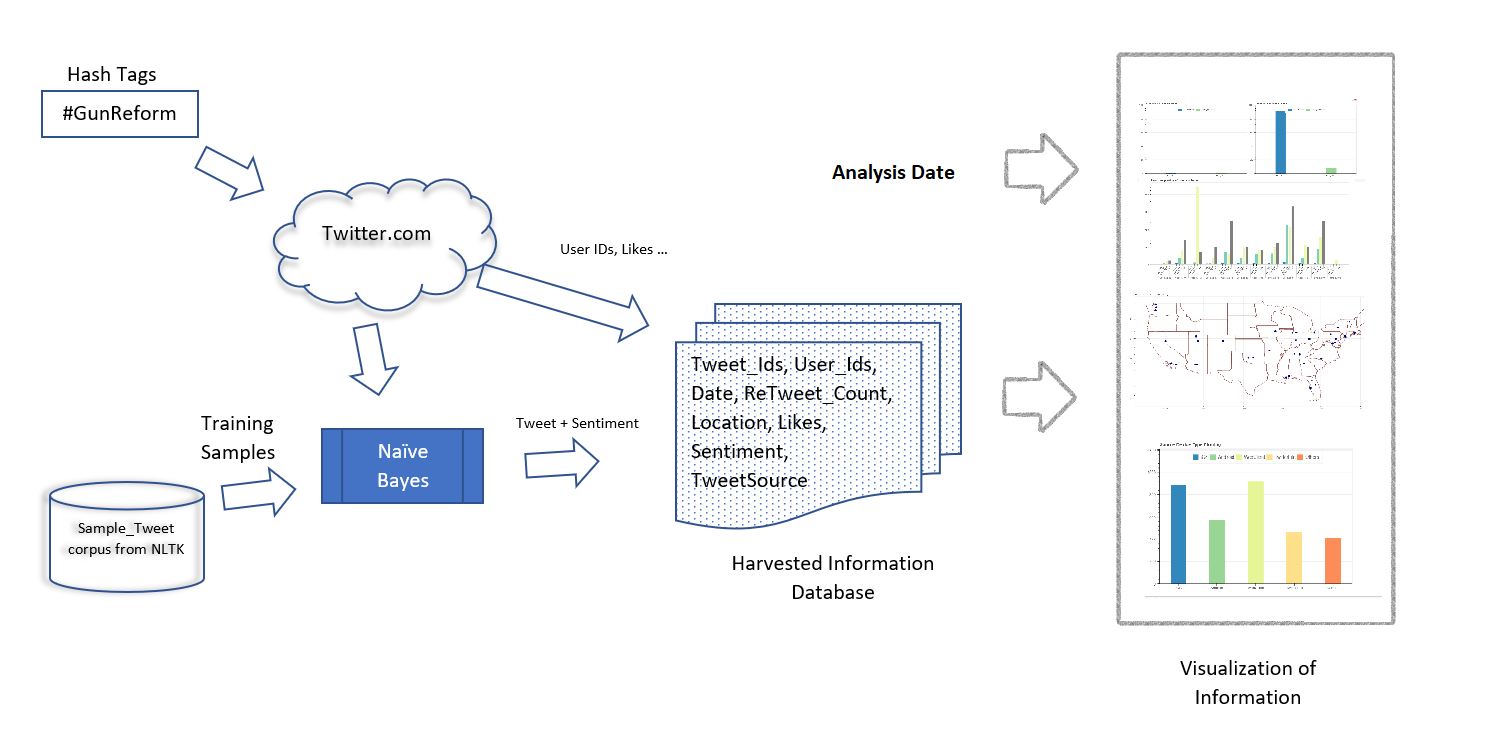
\includegraphics[width=\columnwidth]{Overall_Arch}
% * <vishal.kudale12@gmail.com> 2018-05-02T00:22:14.385Z:
%
% ^.
		% Create a subtitle for the figure.
		\caption{Application Architecture}
		% Define the label of the figure. It's good to use 'fig:title', so you know that the label belongs to a figure.
		\label{fig:tf_plot}
		\end{center}
	\end{figure}
The above diagram depicts overall architecture our project. Following are steps our project will perform.
   \begin{enumerate}
  \item User Enters Hashtag\\ We have provided a text box where user can input all the hashtags on which he wants to perform time-based analysis.
  
  \item Gathering information from twitter and perform sentiment analysis\\
Once we have all the hashtags user want to search, We will query to twitter using tweepy API to get all tweets related to entered  hashtags.

    \item Pre-process data and sentiment analysis\\
Once we have all the information related to hash tags we will extract following fields from it: \\ \\
\texttt{Tweet\_Ids}, \texttt{User\_Ids}, Date, \texttt{ReTweet\_Count}, Location, Likes, Tweet Source, Actual tweets\\ \\
Then we will perform sentiment analysis on tweets and we will store all information along with tweet sentiment in database for further analysis and visualization.
(Detailed information on sentiment analysis is given below)

	\item Acceptance of analysis date from user\\
We have provided a drop-down list from which user can select a date on which user wants to divide gathered information. This division of tweets will be used to analyze the effect of selected date on tweets and user sentiment.

    \item Visualize results\\
Once we have all the processed information we can visualize the results based on date entered by user using graphs such as time series, geo-plot, sentiment analysis bar-graph etc. (Please check visualization section for detailed information).
\end{enumerate}

\section{Data Pre-processing}
	Tweepy API search method returns collection of tweet objects in the json format.\\Extracted fields which are of our interest but some of them were not in the required state. So we did following pre-processing on the data before storing it into CSV file:\\
   \begin{itemize}
  \item Twitter has saved geo-location in bounding box of coordinates which encloses the place. It is series of longitude \& latitude points, defining a box which will contain the place entity this bounding box related to. So, we have taken the average of longitude \& latitude separately to get a single coordinate point.
  \item To get the source of the tweet, we have parsed the ‘source’ attribute from the json \& compared parsed data with specific words like iPhone,Android,Web-client to decide the source of the tweet \& accordingly saved the data as a likert scale.
  \item As retweet count attribute present in the tweet object is same for actual tweet \& retweets of that tweet. So, if we consider retweet count of each tweet object then we will have wrong retweet count. E.g.: Consider a tweet ‘X’ \& ‘Y’ people has retweeted this tweet. In this case, retweet count for X \& all Y will have value as ‘Y’.Here, actual retweet count is Y but if we will get (Y+1)*Y. So, to get the actual retweet count, we first checked each object whether is it a tweet or retweet? If it is tweet then only we considered the retweet count in our data.
\end{itemize}

\section{Sentiment Analysis}
	We are performing sentiment analysis on tweets gathered for some time say 10 years to analyze the effect of various events. We are using Naïve Bayes classification technique to classify each tweet into positive or negative tweet. Along with being simple Naive Bayes is also useful for large datasets.\\
    Using Naïve Bayes Theorem, we can calculate posterior probabilities P(C|X), from class prior probability P(C) and likelihood of each attribute as show in following equation:\\
    \begin{figure}[!hbt]
		% Center the figure.
		\begin{center}
		% Include the eps file, scale it such that it's width equals the column width. You can also put width=8cm for example...
		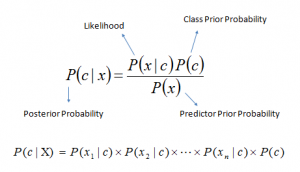
\includegraphics[width=\columnwidth]{Bayes_rule}
% * <vishal.kudale12@gmail.com> 2018-05-02T00:22:14.385Z:
%
% ^.
		% Create a subtitle for the figure.
		\caption{Bayes theorem}
		% Define the label of the figure. It's good to use 'fig:title', so you know that the label belongs to a figure.
		\label{fig:tf_plot}
		\end{center}
	\end{figure}
    \\Above,
   \begin{itemize}
  \item P(c\textbar x) is the posterior probability of target class c given predictor attribute x.
  \item P(c) is the prior probability of target class.
  \item P(x\textbar c) is the likelihood which is the probability of predictor given target class.
  \item P(x) is the prior probability of predictor.
\end{itemize}
Following are key attributes of our sentiment analysis implementation:\\
\begin{enumerate}
  \item Data set\\
We are using \textbf{‘sample\_tweets’} corpus provided by NLTK package for training Naïve Bayes Classifier. This corpus contains total 10000 sample tweets in raw format along with positive and negative sentiment labels. Our code divides these tweets into two parts in 80:20 ratio for training and testing respectively.
  \item Accuracy of Naïve Bayes\\
Our current implementation provides 96\% accuracy on sample\_tweet corpus test set.
\item Preprocessing of raw tweets\\
The data provided in sample\_tweet corpus and data we get from twitter is in raw format and need to be processed before feeding it to classifier. In our current implementation we are taking care of following cases:\\
\begin{enumerate}
  \item Emoticons( E.g. : ) : )) etc.)
  \item StopWords ( E.g. A, An, The etc.)
  \item Case Sensitivity
  \item URLs, Hashtags, Usernames
  \item White Spaces and Repeating Characters
\end{enumerate}
\item Feature selection and training\\
We are using most common words found in training set as feature for our classifier. Along with most common words we are converting URLs, Hashtags and emoticons into keywords and feeding it to Naive Bayes classifier. We believe that emoticons are great indicator of user’s emotion and should be used for sentiment analysis.
\item Train once approach\\
As everyone knows, training classifier is time consuming task. Hence our code comes with pre trained classifier trained  on sample\_tweets corpus saved in pickle object. Also, we allow user to retrain the classifier. Once retraining is done we save trained classifier in pickle object in classifier folder. So whenever user inputs new hashtags for analysis our code will pick up stored classifier saving us from wasting time on training phase.
\end{enumerate}

\section{Visualization}
As mentioned above in abstract, this implementation allows to perform analysis on any event, public concern, or any ongoing discussion on social platform. User can provide respective tweet hashtag in input and the follow steps to get the detailed results.\\
\begin{figure}[!hbt]
		% Center the figure.
		\begin{center}
		% Include the eps file, scale it such that it's width equals the column width. You can also put width=8cm for example...
		
\includegraphics[width=\columnwidth]{Screen_Shot_2018-05-01_at_7_19_58_PM}
% * <vishal.kudale12@gmail.com> 2018-05-02T00:22:14.385Z:
%
% ^.
		% Create a subtitle for the figure.
		\caption{Input Box for user}
		% Define the label of the figure. It's good to use 'fig:title', so you know that the label belongs to a figure.
		\label{fig:tf_plot}
		\end{center}
	\end{figure}
    \\You can use above mentioned text input to specify the hashtag for which you want to perform the analysis. Once you provide that and run remaining cell in jupyter notebook, you will get the all the charts at the end. Here due to twitter api restriction we can only extract data for last 10 days. Because of that all the results mentioned below are generated on data extracted for \#GunReform for last 10 days.\\
    List of graphs generated as part of this analysis
   \begin{enumerate}
  \item Time Series Analysis for Sentiment plot\\ This graph shows how people’s views and sentiments changes with respect to time.
  \begin{figure}[!hbt]
		% Center the figure.
		\begin{center}
		% Include the eps file, scale it such that it's width equals the column width. You can also put width=8cm for example...
		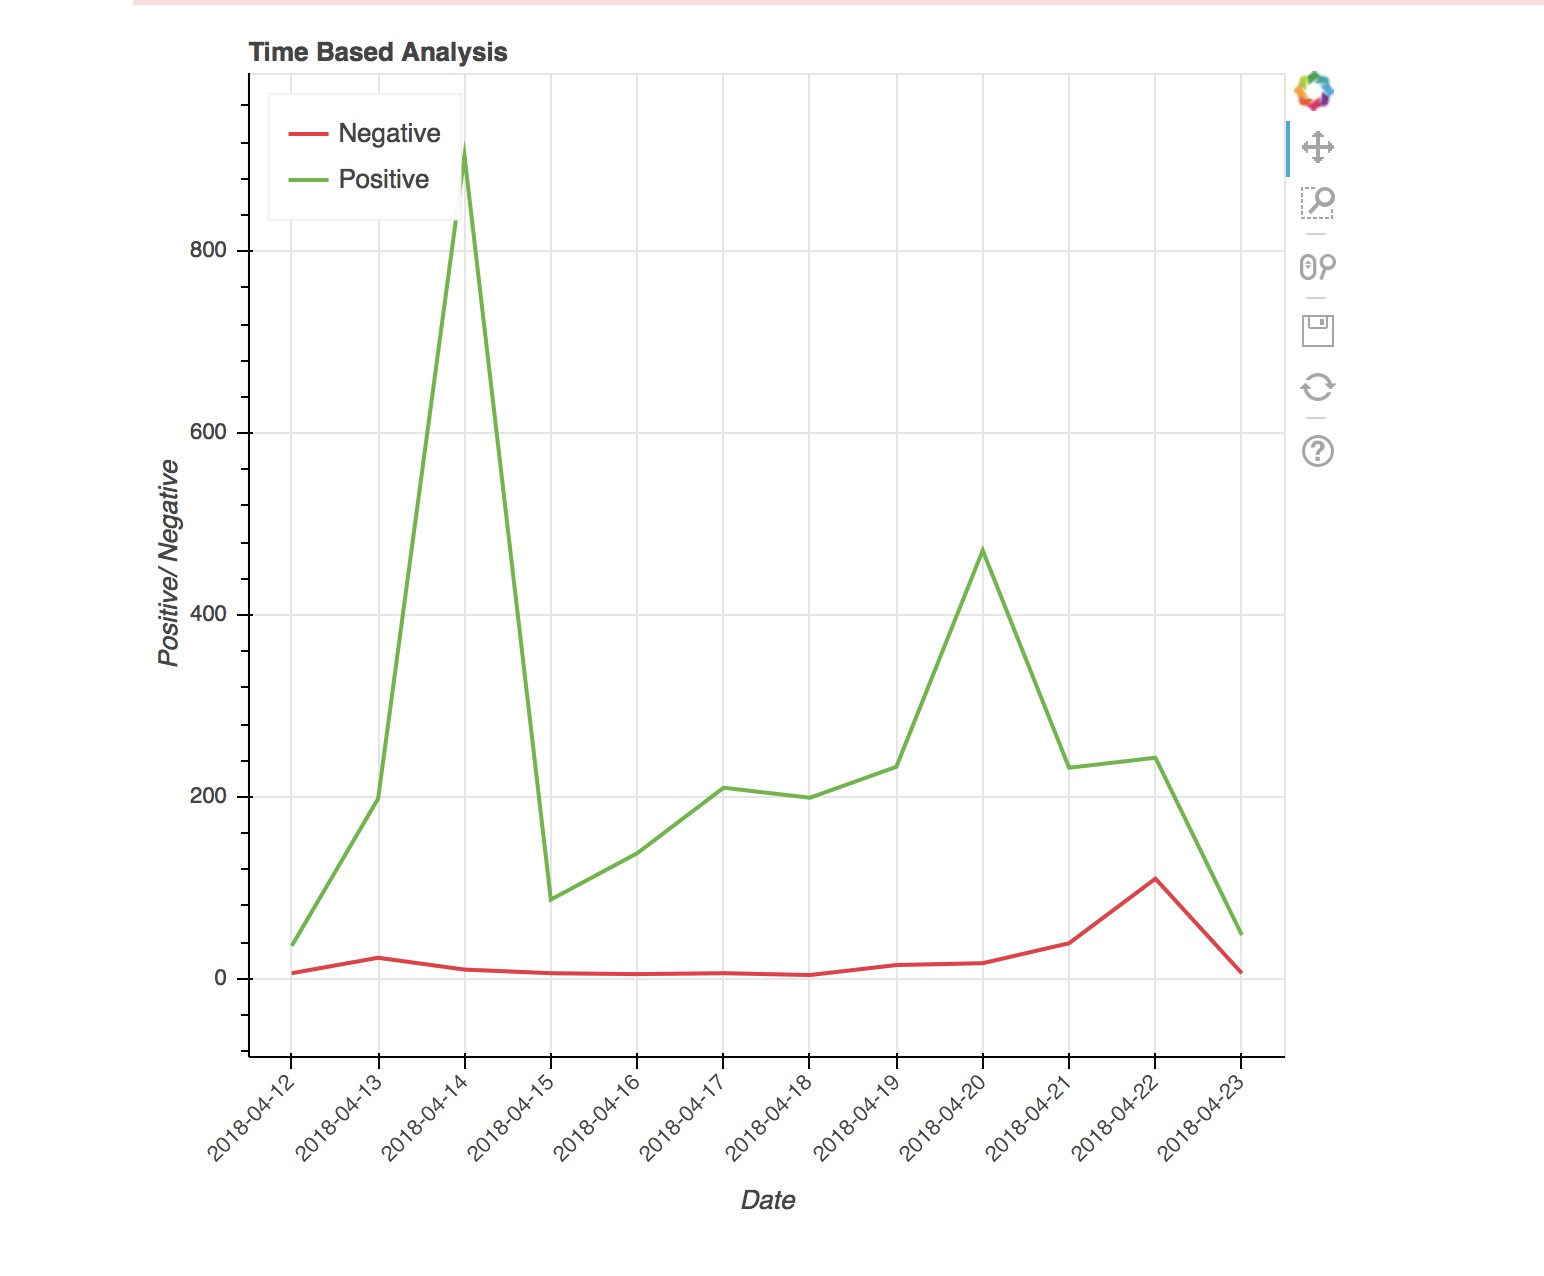
\includegraphics[width=\columnwidth]{Screen_Shot_2018-05-01_at_7_17_45_PM}
% * <vishal.kudale12@gmail.com> 2018-05-02T00:22:14.385Z:
%
% ^.
		% Create a subtitle for the figure.
		\caption{Time Series Analysis}
		% Define the label of the figure. It's good to use 'fig:title', so you know that the label belongs to a figure.
		\label{fig:tf_plot}
		\end{center}
	\end{figure}
    \\As you can see graph in Fig.4, contains date wise analysis of positive and negative tweets. This time series data allows us to understand the trend of tweets with respect of time and their sentiments. By visualizing time series data we can say whether people have same sentiment throughout the entire time or it has changes, whether it become more positive or negative,  Is there any spikes in daily results due to some event. As you can see in result we have data from April 12th to April 23rd 2018. From this plot we can say that people have positive views when it comes to strict gun reform. More number of positive tweets then compare to negative tweets.
  
  \item Before-After analysis plot\\ To see what was the response of people before and after certain date. 
  \begin{figure}[!hbt]
		% Center the figure.
		\begin{center}
		% Include the eps file, scale it such that it's width equals the column width. You can also put width=8cm for example...
		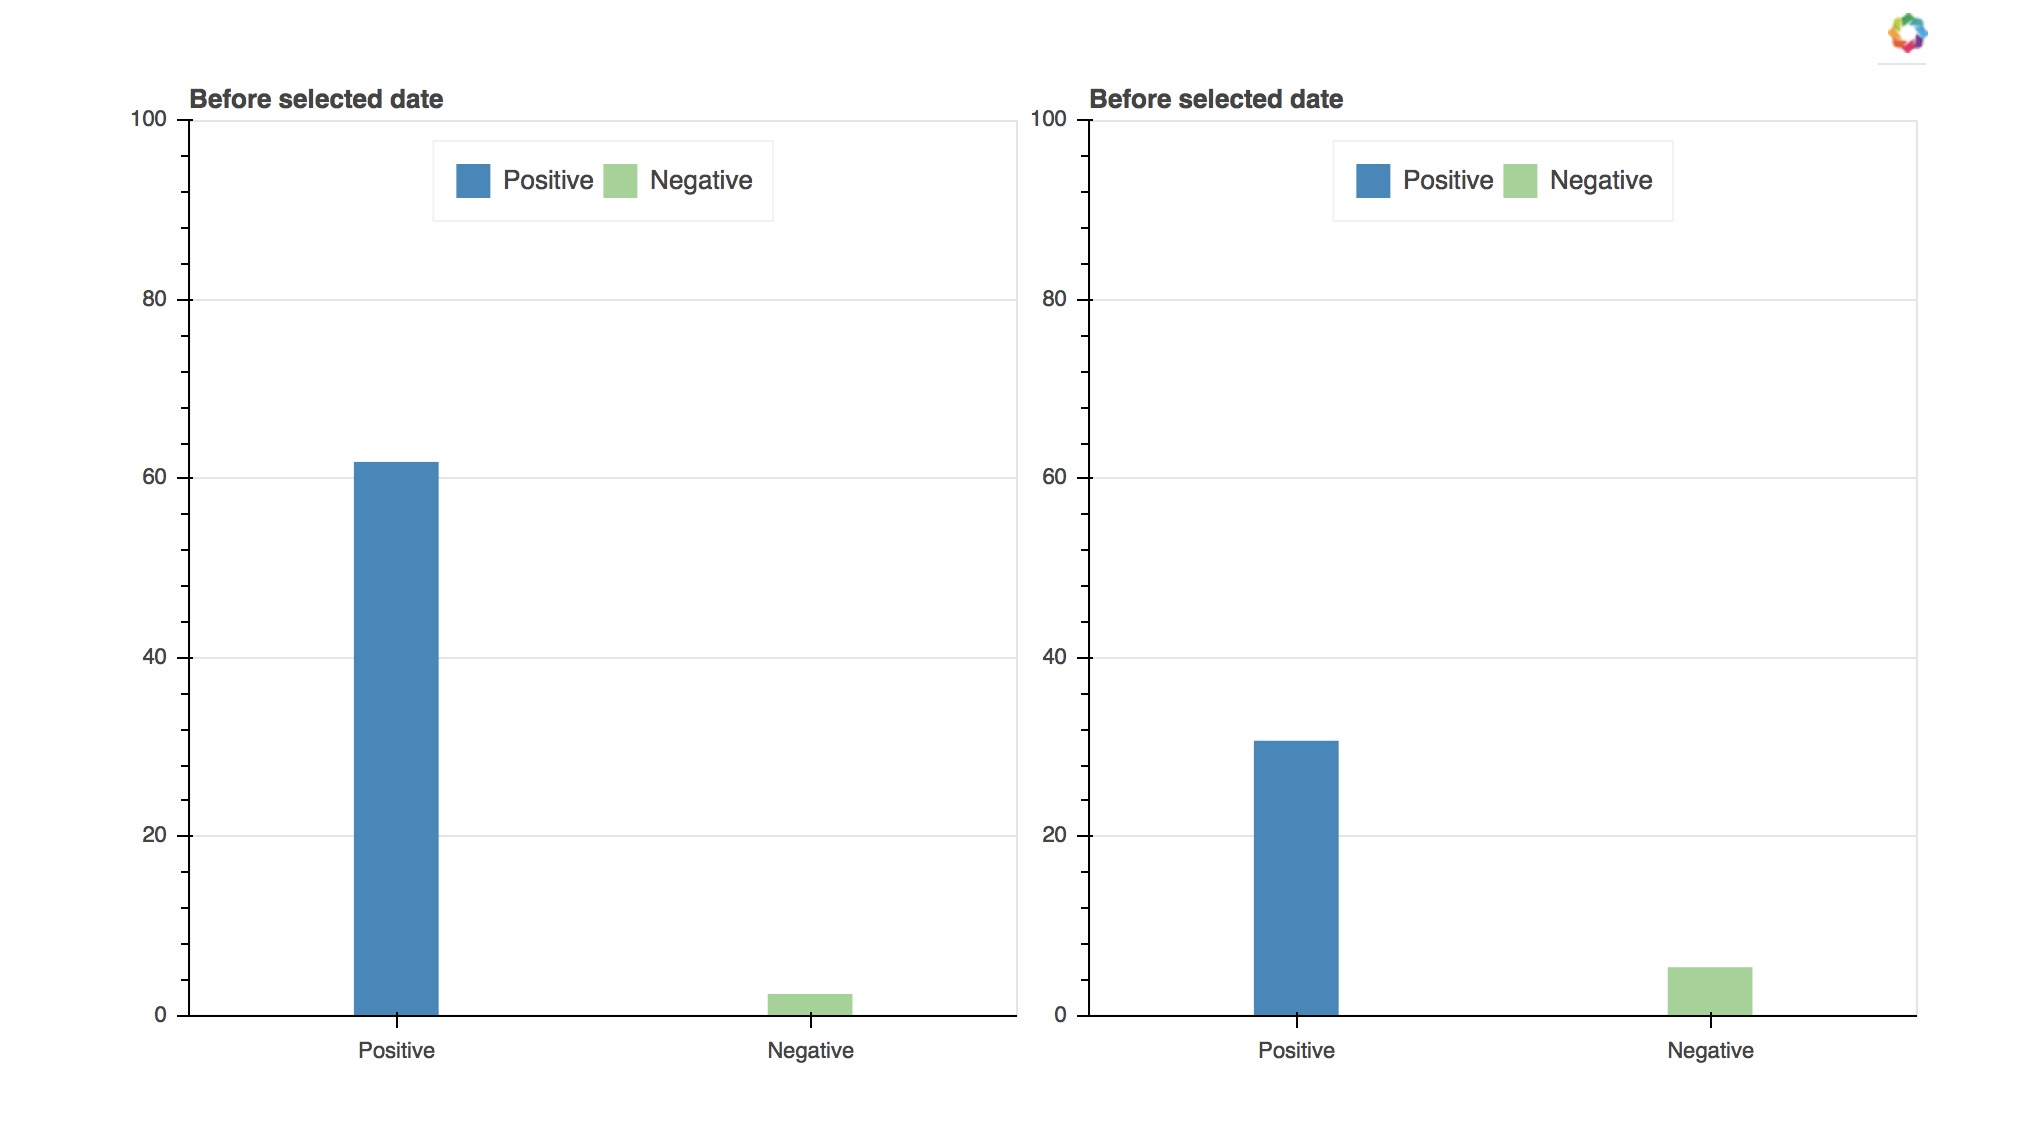
\includegraphics[width=\columnwidth]{Screen_Shot_2018-05-01_at_7_17_10_PM}
% * <vishal.kudale12@gmail.com> 2018-05-02T00:22:14.385Z:
%
% ^.
		% Create a subtitle for the figure.
		\caption{Date based Before-After analysis }
		% Define the label of the figure. It's good to use 'fig:title', so you know that the label belongs to a figure.
		\label{fig:tf_plot}
		\end{center}
	\end{figure}
    
    \begin{figure}[!hbt]
		% Center the figure.
		\begin{center}
		% Include the eps file, scale it such that it's width equals the column width. You can also put width=8cm for example...
		
\includegraphics[width=\columnwidth]{Screen_Shot_2018-05-01_at_7_17_24_PM}
% * <vishal.kudale12@gmail.com> 2018-05-02T00:22:14.385Z:
%
% ^.
		% Create a subtitle for the figure.
		\caption{Date Selection drop-down}
		% Define the label of the figure. It's good to use 'fig:title', so you know that the label belongs to a figure.
		\label{fig:tf_plot}
		\end{center}
	\end{figure}
    One of our hypothesis that certain event can have impact on views of people. Ex. Shootout at a school might lead increase in tweets related to strict gun reform act with positive sentiments. On  that hypothesis we build this graph such that if we want to see how people were reacting on twitter before and after certain date for a given issue. By selecting date from drop down two graphs will be generated dynamically. Both containing total number of positive and negative tweets.
    \item Date-wise plotting of twitter attributes\\ Get day by day analysis of attributes like, Total number of tweets, Retweets, Likes and how many unique user have tweeted that day.
    \begin{figure}[!hbt]		
		\begin{center}		
		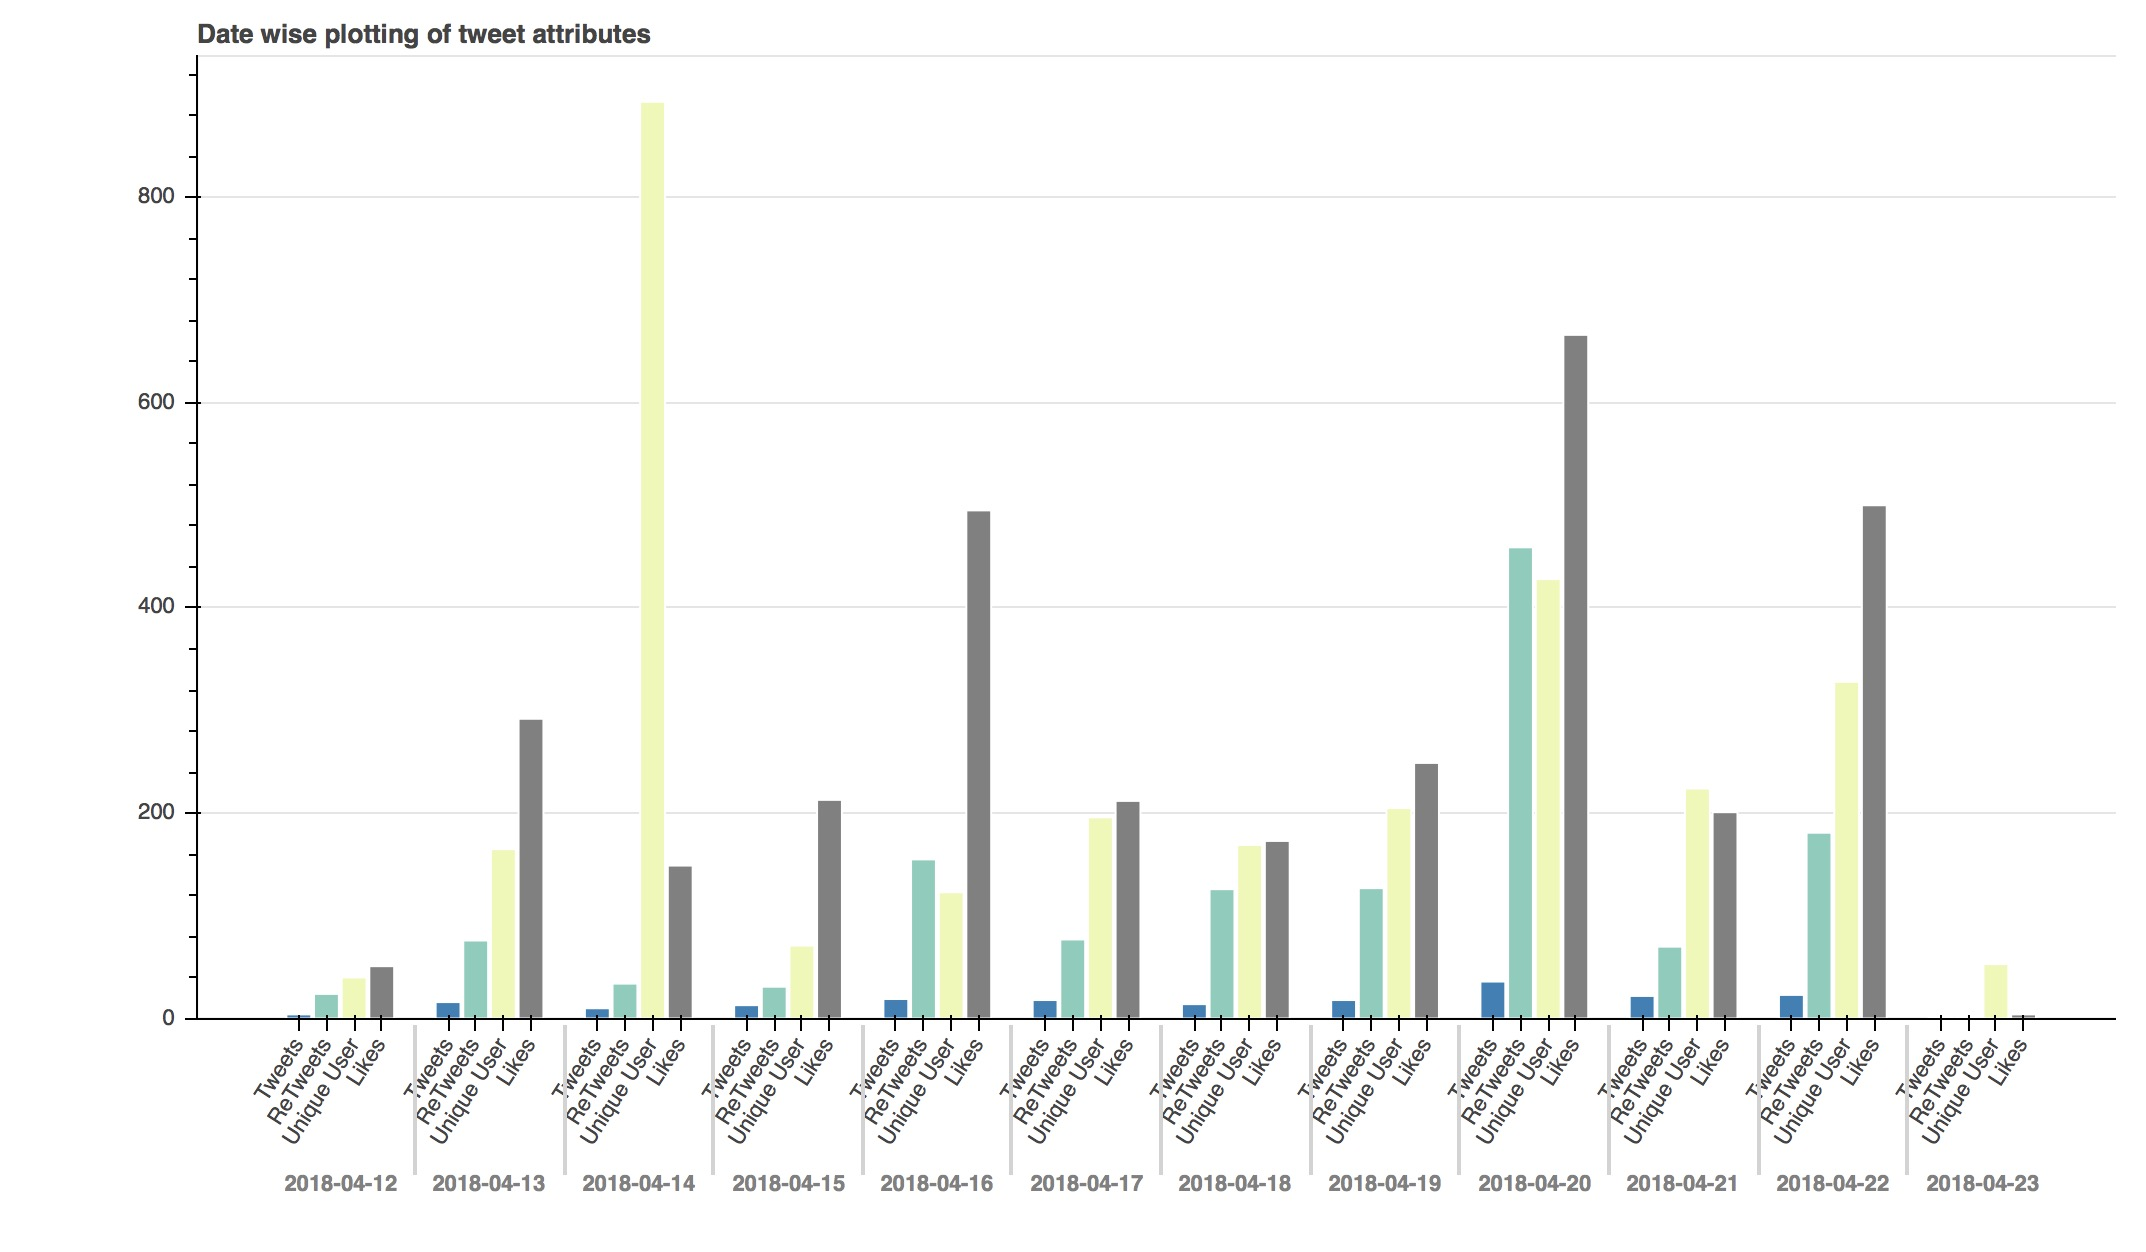
\includegraphics[width=\columnwidth]{Screen_Shot_2018-05-01_at_7_17_36_PM}
		\caption{Date based comparison of twitter attributes}		
		\label{fig:tf_plot}
		\end{center}
	\end{figure}
    \\This plot is used to get general information like how many tweets, and retweets related to specific topic on given day along with likes for tweets and retweets. Also this plot contains list of unique user. This will help to analyze  the trend how new people reacting to specific problem. This statistical information is helpful to get a clear picture on how many people are involved, concerned and actively taking participation on given discussion.
\\This will help us to understand how much people are interested in given issue. Also how many new people have joined to express their feelings on twitter. 

    \item User Location Plot\\ To see whether people from specific region is tweeting about given issue or people across united states are actively participating in given discussion.
    \begin{figure}[!hbt]		
		\begin{center}		
		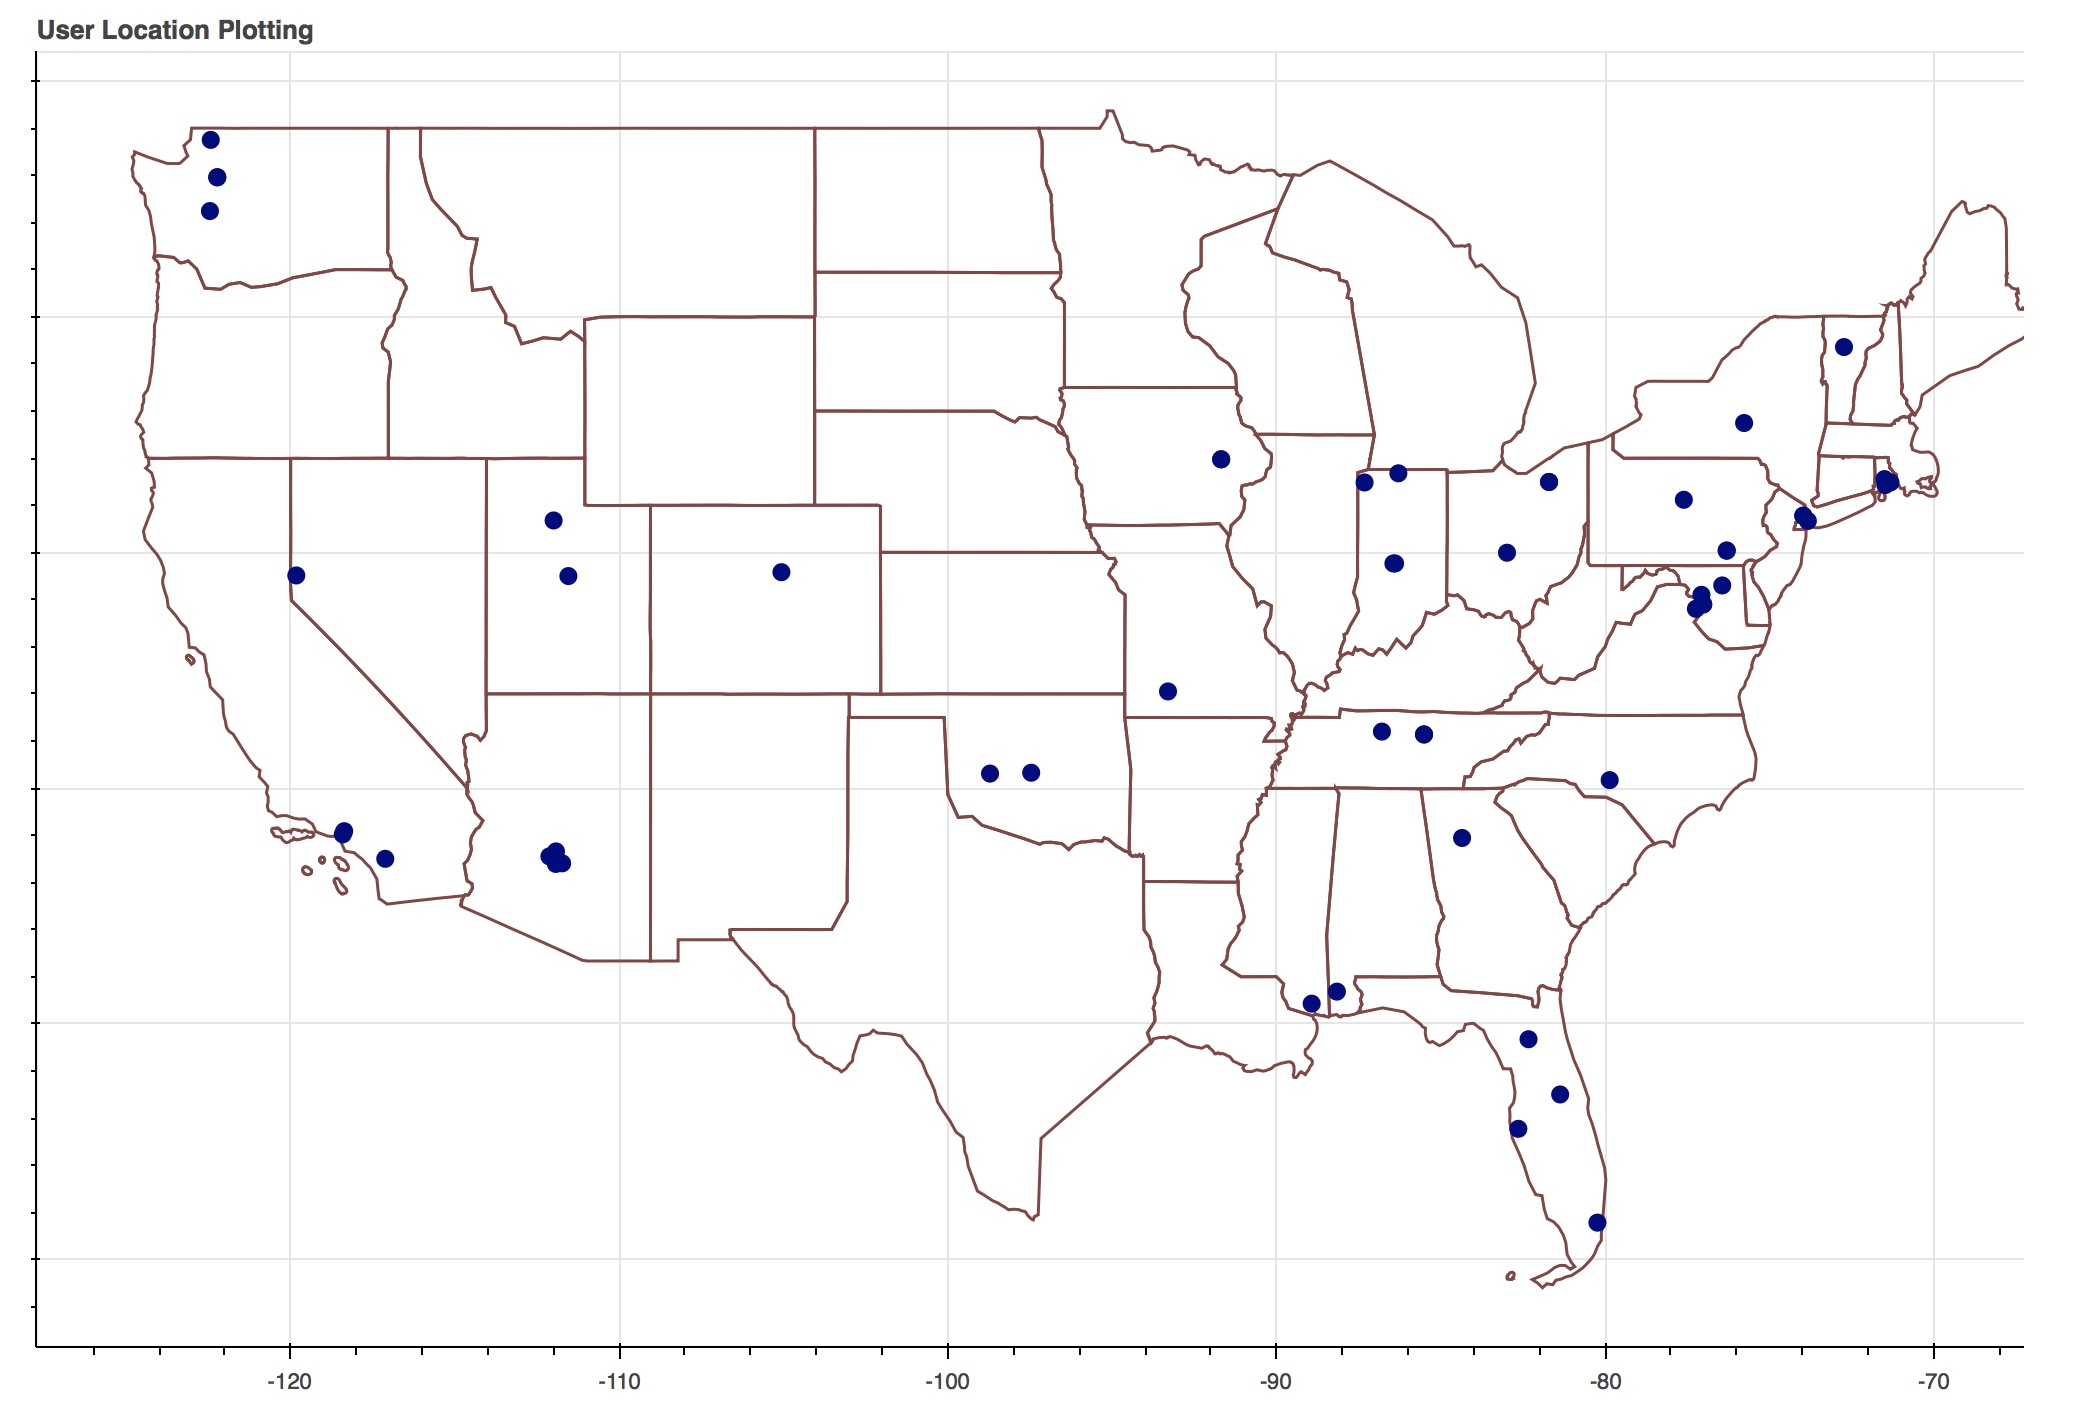
\includegraphics[width=\columnwidth]{Screen_Shot_2018-05-01_at_7_17_59_PM}
		\caption{User's Location Mapping}		
		\label{fig:tf_plot}
		\end{center}
	\end{figure}
    \\To access the location on twitter user has to enable location sharing. Once its enabled twitter stores the location where given tweet was tweeted.This will help us to understand awareness of people with respect to given problem also to track location wise activity of people on twitter. 
As mentioned above twitter api will only generate data for last 15 days also less people allow access to their locations, because of that we only managed to plot few of the tweet origin. But with enterprise twitter api with same code we can get more tweets and get more data points on given plot.

	\item Source Device Plot\\ Plot the source of device used to tweet.
    \begin{figure}[!hbt]		
		\begin{center}		
		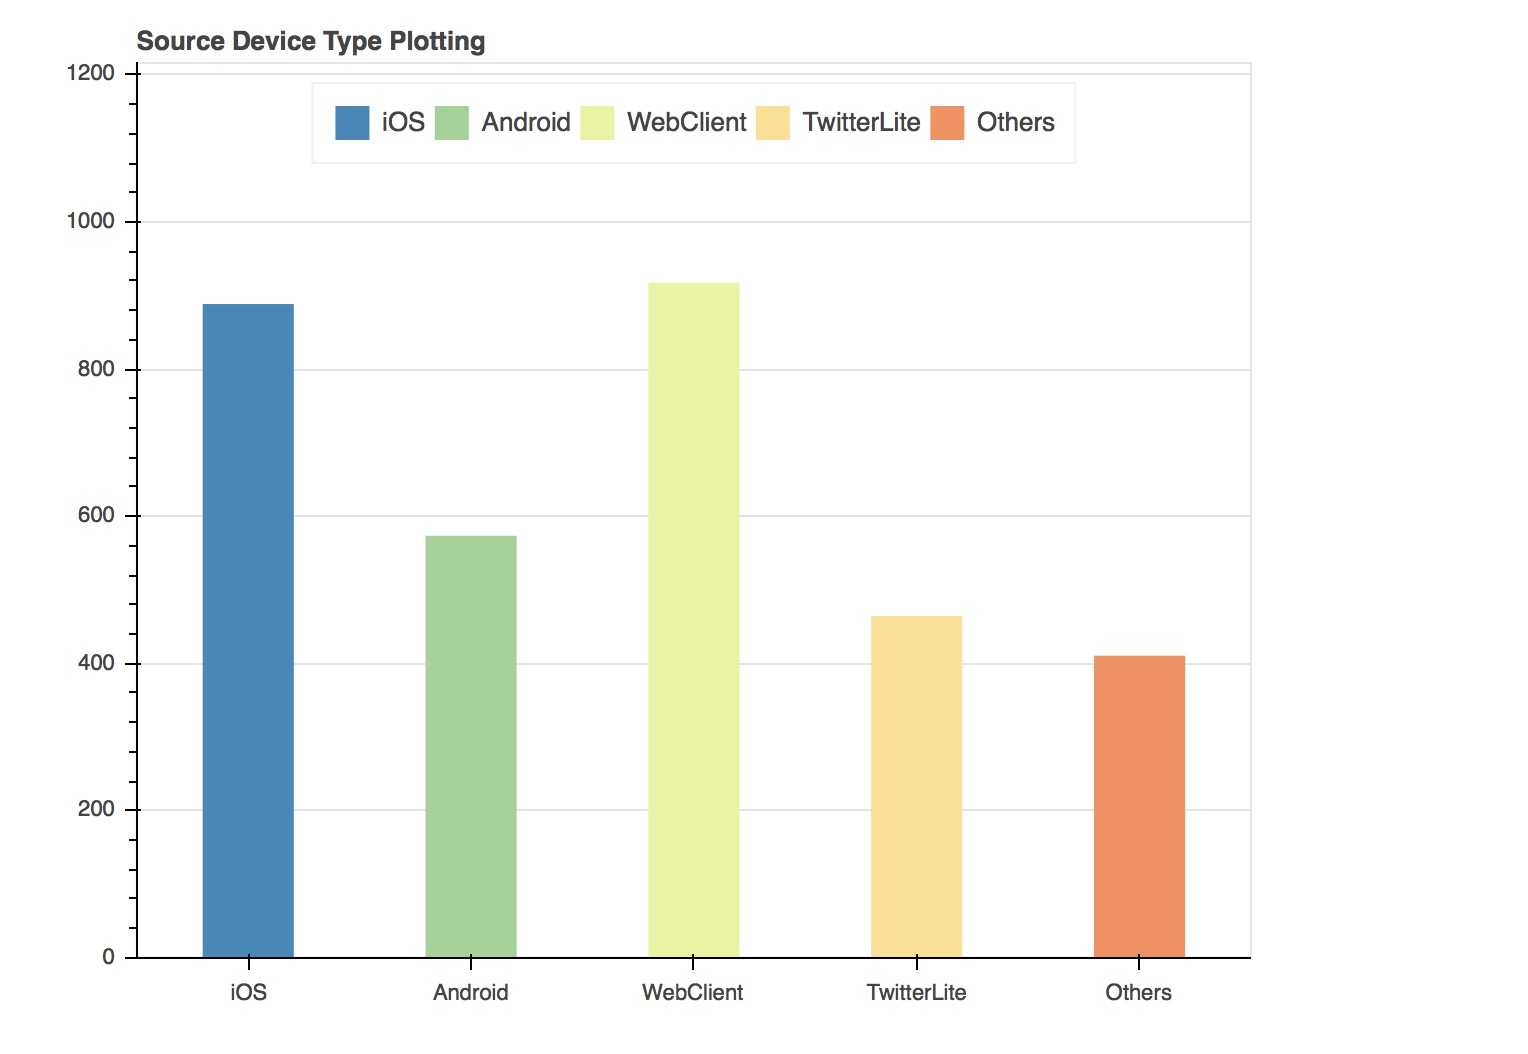
\includegraphics[width=\columnwidth]{Screen_Shot_2018-05-01_at_7_18_08_PM}
		\caption{Devices used to tweet }		
		\label{fig:tf_plot}
		\end{center}
	\end{figure}
    \\This will give us an technical aspect of analysis. What medium people use to reach out to outer world to express their concerns. To see whether people use phones to tweet or they use webportal to express their concerns. Android, IOS app and Twitter Lite can be accessed via phone. From graph we can say that more number of people use mobile device to tweet compare to personal computer as they are handy now a days.
    \item Total Positive-Negative Sentiment Plot\\ This is a plot that consider sentiments for  all the tweets related to a topic so far to visualize whether the overall response is positive or negative.
    \begin{figure}[!hbt]		
		\begin{center}		
		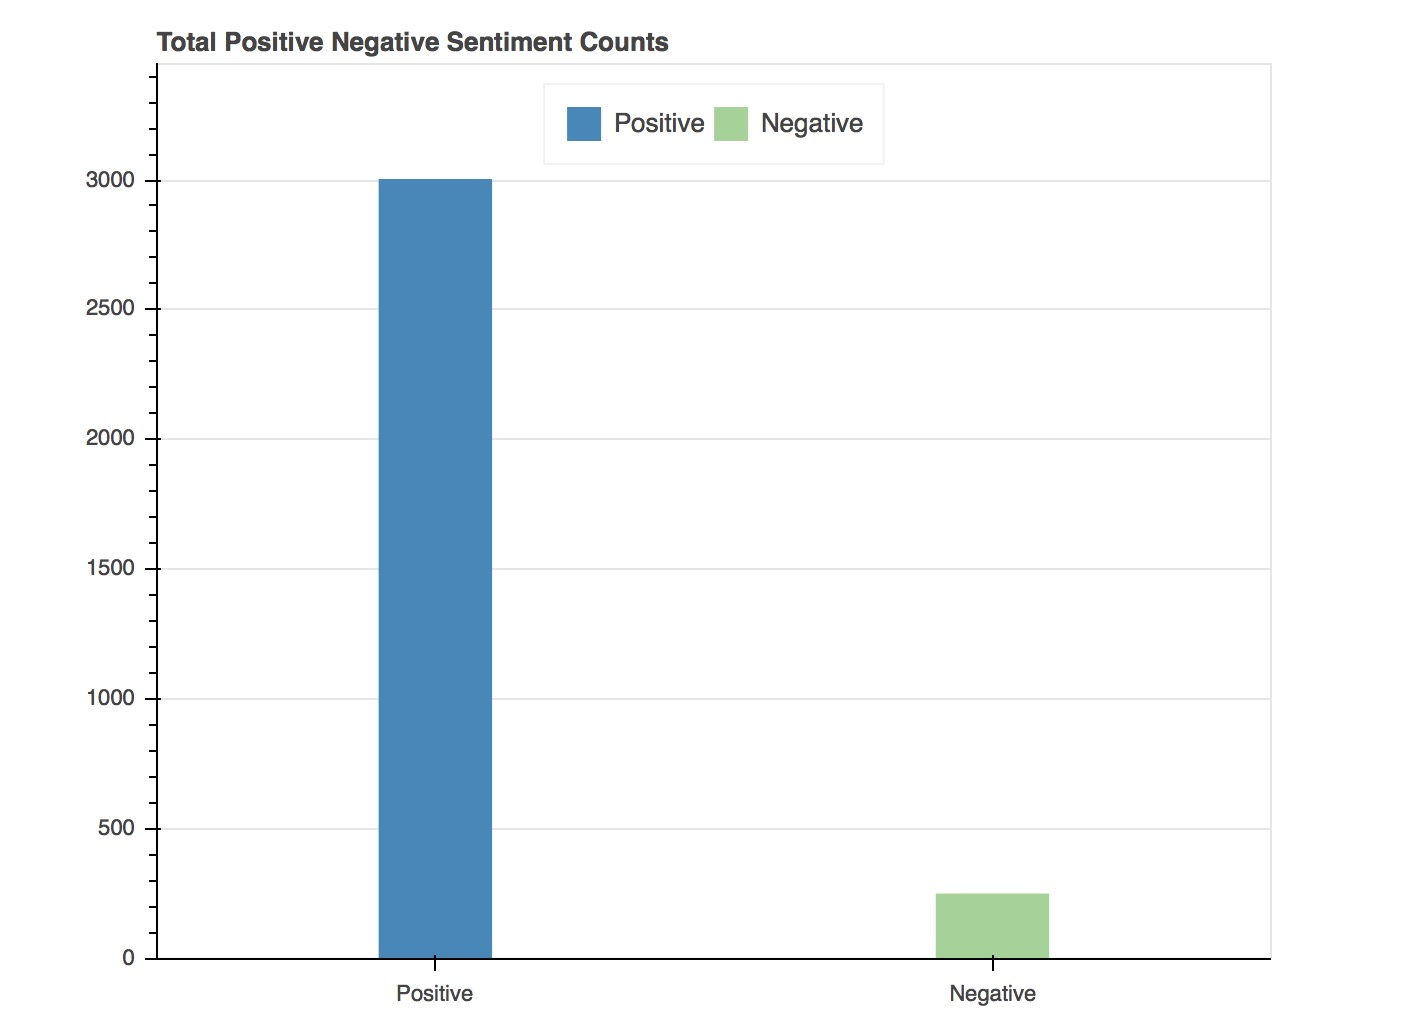
\includegraphics[width=\columnwidth]{Screen_Shot_2018-05-01_at_7_18_18_PM}
		\caption{Overall Sentiment Analysis }		
		\label{fig:tf_plot}
		\end{center}
	\end{figure}
    \\Fig. 10. gives details on overall response of people for given time frame by ploing total positive and negative tweets.From this we can say that there are more number of positive tweets compare to negative tweets.  
\end{enumerate}

\section{Technical Details}
\begin{itemize}
  \item Packages used
  	\begin{enumerate}
 		 \item Bokeh\\ We have used ‘Bokeh 0.12.7’ version. We have used bokeh to take user input from user. We have used it to display different plots like time-series plot, bar charts, geo-location plot.
  		\item Tweepy Library\\ We have used Tweepy library to extract the tweet related data from Twitter.
        \item NLTK Library\\ This library is used to train our classifier based on twitter\_sample data. It is also used to perform sentiment analysis over the tweets extracted from twitter based on user’s input.

	\end{enumerate}
  \item Dependencies\\
  Our application is dependent on following:
  \begin{enumerate}
		\item 	Bokeh
 		\item 	Numpy
		\item	Blaze
		\item	Dask
		\item	Pandas
		\item	JsonPickle	
		\item	Tweepy
		\item	NLTK
\end{enumerate}
Run following commands to install above dependencies on Anaconda Prompt:
	\begin{enumerate}
		\item 	python -m bokeh info \\ conda uninstall bokeh \\ conda install bokeh=0.12.7
 		\item 	conda install NumPy
		\item	conda install blaze
		\item	conda install dask
		\item	conda install pandas
		\item	pip install jsonpickle	
		\item	pip install tweepy
		\item	pip install -U nltk
\end{enumerate}
\end{itemize}

\section{Issues faced}
Twitter api(Tweepy) has access to data just for last 10 days.So we have changed our scope of the project from overall analysis to analysis on available last 10 days data.

\section{Conclusion}
	We are able to perform a sentiment analysis on extracted twitter data based on the submitted query(hashtag) by user. Also We have represented all sentiment results in the form of  time-series graph \& bar charts. With the help of these output, one can definitely decide responses of people from all over the world to given query i.e. one can easily say whether people’s response is positive by just by observing the output plots. From our analysis, there is a positive response from people for gun-reform act law. People are using mobile devices than web-client to tweet their thoughts. It is not the case that people are active only from the place where gun-shooting incidents are happened but people are active all over the United States. Also, it is not the case that only some people are just tweeting/retweeting about gun-reform act. There are some new people who also tweets on it.

% Now we need a bibliography:
\begin{thebibliography}{5}

	%Each item starts with a \bibitem{reference} command and the details thereafter.
	\bibitem{1} % Web document
		\url{https://www.analyticsvidhya.com/blog/2017/09/naive-bayes-explained/}
	\bibitem{2}
    	\url{http://docs.tweepy.org/en/v3.5.0/}
    \bibitem{3}
    	\url{http://bokeh.pydata.org/en/0.9.3/docs/user_guide/charts.html}        
    \bibitem{4}
    	\url{https://bokeh.pydata.org/en/latest/}
\end{thebibliography}

% Your document ends here!
\end{document}